\documentclass[tikz,border=2pt]{standalone}
\usepackage{pgfplots}
\usetikzlibrary{shapes.geometric, intersections, calc}
\pgfplotsset{compat=1.7}

\begin{document}
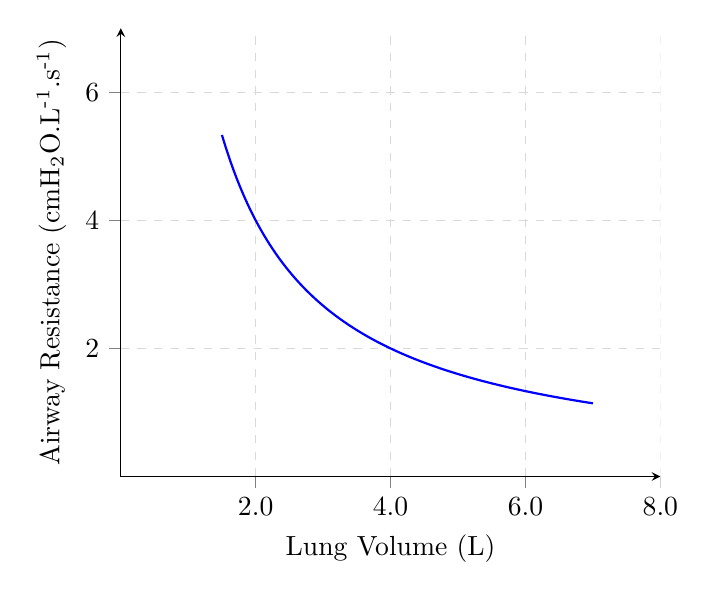
\begin{tikzpicture}[dot/.style={circle,inner sep=1pt,fill,label={#1},name=#1},
 extended line/.style={shorten >=-#1,shorten <=-#1},
 extended line/.default=10cm]

\tikzset{
    myarrow/.style={
        sloped,
        isosceles triangle,
        anchor=apex,
        fill=black,
        inner sep=2pt
    }
}

\makeatletter
\def\parsenode[#1]#2\pgf@nil{%
    \tikzset{label node/.style={#1}}
    \def\nodetext{#2}
}

\tikzset{
    add node at x/.style 2 args={
        name path global=plot line,
        /pgfplots/execute at end plot visualization/.append={
                \begingroup
                \@ifnextchar[{\parsenode}{\parsenode[]}#2\pgf@nil
            \path [name path global = position line #1-1]
                ({axis cs:#1,0}|-{rel axis cs:0,0}) --
                ({axis cs:#1,0}|-{rel axis cs:0,1});
            \path [xshift=1pt, name path global = position line #1-2]
                ({axis cs:#1,0}|-{rel axis cs:0,0}) --
                ({axis cs:#1,0}|-{rel axis cs:0,1});
            \path [
                name intersections={
                    of={plot line and position line #1-1},
                    name=left intersection
                },
                name intersections={
                    of={plot line and position line #1-2},
                    name=right intersection
                },
                label node/.append style={pos=1}
            ] (left intersection-1) -- (right intersection-1)
            node [label node]{\nodetext};
            \endgroup
        }
    },
    add node at y/.style 2 args={
        name path global=plot line,
        /pgfplots/execute at end plot visualization/.append={
                \begingroup
                \@ifnextchar[{\parsenode}{\parsenode[]}#2\pgf@nil
            \path [name path global = position line #1-1]
                ({axis cs:0,#1}-|{rel axis cs:0,0}) --
                ({axis cs:0,#1}-|{rel axis cs:1,1});
            \path [yshift=1pt, name path global = position line #1-2]
                ({axis cs:0,#1}-|{rel axis cs:0,0}) --
                ({axis cs:0,#1}-|{rel axis cs:1,1});
            \path [
                name intersections={
                    of={plot line and position line #1-1},
                    name=left intersection
                },
                name intersections={
                    of={plot line and position line #1-2},
                    name=right intersection
                },
                label node/.append style={pos=1}
            ] (left intersection-1) -- (right intersection-1)
            node [label node] {\nodetext};
            \endgroup
        }
    }
}
\makeatother
    \begin{axis}[
        axis x line=middle,
        axis y line=middle,
        x tick label style={/pgf/number format/fixed,
                            /pgf/number format/fixed zerofill,
                            /pgf/number format/precision=1},
        y tick label style={/pgf/number format/fixed,
                            /pgf/number format/fixed zerofill,
                            /pgf/number format/precision=0},
        grid = major,
        grid style={dashed, gray!30},
    	  x label style={at={(axis description cs:0.5,-0.1)},anchor=north},
	  y label style={at={(axis description cs:-0.1,.5)},rotate=90,anchor=south},
        xmin=0,
        xmax= 8,
        ymin= 0,
        ymax= 7,
	 ylabel near ticks,
	xlabel near ticks,
        xlabel=Lung Volume (L),
        ylabel=Airway Resistance (cmH\textsubscript{2}O.L\textsuperscript{-1}.s\textsuperscript{-1}),
        tick align=outside,
        enlargelimits=false]
	\coordinate (o) (0,0);

	\addplot[domain=1.5:7, blue, thick,samples=500] {(8/x)};
\end{axis}


\end{tikzpicture} 
\end{document}